
\documentclass[12pt]{article}


\usepackage{latexsym}
\usepackage[english,finnish]{babel}
\usepackage{bbm}
\usepackage{mathrsfs}
\usepackage{ifthen}
\usepackage{url}
\usepackage{enumerate}
\usepackage{fancyhdr}
% AMS packages:
\usepackage{amsbsy}
\usepackage{amsfonts}
\usepackage{amsmath}
\usepackage{amssymb}
\usepackage{amsthm}
\usepackage{amsxtra}
% for comments to work
\usepackage{verbatim}
\usepackage{graphicx}

\newcommand{\pat}{\partial}
\newcommand{\be}{\begin{equation}}
\newcommand{\ee}{\end{equation}}
\newcommand{\bea}{\begin{eqnarray}}
\newcommand{\eea}{\end{eqnarray}}
\newcommand{\abf}{{\bf a}}
\newcommand{\Zcal}{{\cal Z}_{12}}
\newcommand{\zcal}{z_{12}}
\newcommand{\Acal}{{\cal A}}
\newcommand{\Fcal}{{\cal F}}
\newcommand{\Ucal}{{\cal U}}
\newcommand{\Vcal}{{\cal V}}
\newcommand{\Ocal}{{\cal O}}
\newcommand{\Rcal}{{\cal R}}
\newcommand{\Scal}{{\cal S}}
\newcommand{\Lcal}{{\cal L}}
\newcommand{\Hcal}{{\cal H}}
\newcommand{\hsf}{{\sf h}}
\newcommand{\half}{\frac{1}{2}}
\newcommand{\Xbar}{\bar{X}}
\newcommand{\xibar}{\bar{\xi }}
\newcommand{\barh}{\bar{h}}
\newcommand{\Ubar}{\bar{\cal U}}
\newcommand{\Vbar}{\bar{\cal V}}
\newcommand{\Fbar}{\bar{F}}
\newcommand{\zbar}{\bar{z}}
\newcommand{\wbar}{\bar{w}}
\newcommand{\zbarhat}{\hat{\bar{z}}}
\newcommand{\wbarhat}{\hat{\bar{w}}}
\newcommand{\wbartilde}{\tilde{\bar{w}}}
\newcommand{\barone}{\bar{1}}
\newcommand{\bartwo}{\bar{2}}
\newcommand{\nbyn}{N \times N}
\newcommand{\repres}{\leftrightarrow}
%\newcommand{\Tr}{{\rm Tr}}
%\newcommand{\tr}{{\rm tr}}
\newcommand{\ninfty}{N \rightarrow \infty}
\newcommand{\unitk}{{\bf 1}_k}
\newcommand{\unitm}{{\bf 1}}
\newcommand{\zerom}{{\bf 0}}
\newcommand{\unittwo}{{\bf 1}_2}
\newcommand{\holo}{{\cal U}}
\newcommand{\bra}{\langle}
\newcommand{\ket}{\rangle}
\newcommand{\muhat}{\hat{\mu}}
\newcommand{\nuhat}{\hat{\nu}}
\newcommand{\rhat}{\hat{r}}
\newcommand{\phat}{\hat{\phi}}
\newcommand{\that}{\hat{t}}
\newcommand{\shat}{\hat{s}}
\newcommand{\zhat}{\hat{z}}
\newcommand{\what}{\hat{w}}
\newcommand{\sgamma}{\sqrt{\gamma}}
\newcommand{\bfE}{{\bf E}}
\newcommand{\bfB}{{\bf B}}
\newcommand{\bfM}{{\bf M}}
\newcommand{\cl} {\cal l}
\newcommand{\ctilde}{\tilde{\chi}}
\newcommand{\ttilde}{\tilde{t}}
\newcommand{\ptilde}{\tilde{\phi}}
\newcommand{\utilde}{\tilde{u}}
\newcommand{\vtilde}{\tilde{v}}
\newcommand{\wtilde}{\tilde{w}}
\newcommand{\ztilde}{\tilde{z}}

% misc
\newcommand{\vc}[1]{\mathbf{#1}}
\newcommand{\defem}[1]{{\em #1\/}}
\newcommand{\vep}{\varepsilon}
\newcommand{\wto}{\overset{{\rm w}}{\to}}
\newcommand{\sto}{\overset{{\rm s}}{\to}}
\DeclareMathOperator{\wlim}{w-lim}
\DeclareMathOperator{\slim}{s-lim}
\DeclareMathOperator{\tr}{Tr}

\newcommand{\qand}{\quad\text{and}\quad}

% To define sets:
\newcommand{\defset}[2]{ \left\{ #1 \left|\, #2\makebox[0pt]{$\displaystyle\phantom{#1}$}\right.\!\right\} }

\newcounter{alplisti}
\renewcommand{\thealplisti}{\alph{alplisti}}
\newenvironment{alplist}[1][(\thealplisti)]{\begin{list}{{\rm #1}\ }{ %
      \usecounter{alplisti} %
    \setlength{\itemsep}{0pt}
    \setlength{\parsep}{0pt}  %
%    \setlength{\leftmargin}{5em} %
%    \setlength{\labelwidth}{5em} %
%    \setlength{\labelsep}{1em} %
%    \settowidth{\labelwidth}{(DR2)}
     \setlength{\topsep}{0pt} %
}}{\end{list}}

% Norms:
\newcommand{\abs}[1] {\lvert #1 \rvert}
\newcommand{\norm}[1]{\lVert #1 \rVert}
\newcommand{\floor}[1] {\lfloor {#1} \rfloor}
\newcommand{\ceil}[1]  {\lceil  {#1} \rceil}

% Basic spaces
\newcommand{\R} {\mathbb{R}}
\newcommand{\C} {{\mathbb{C}}}
\newcommand{\Rd} {{\mathbb{R}^{d}}}
\newcommand{\N} {\mathbb{N}}
\newcommand{\Z} {\mathbb{Z}}
\newcommand{\Q} {\mathbb{Q}}
\newcommand{\K} {\mathbb{K}}
\newcommand{\T} {\mathbb{T}}


\hoffset 0.5cm
\voffset -0.4cm
\evensidemargin -0.2in
\oddsidemargin -0.2in
\topmargin -0.2in
\textwidth 6.3in
\textheight 8.4in

\begin{document}

\normalsize

\baselineskip 14pt

\begin{center}
{\Large {\bf FYMM/MMP IIIa \ \ \ \ \ \ \ Solutions to Course Project \ \  Oct 26 2030}}
Jake Muff
Student number: 015361763
\end{center}

\bigskip

\enlargethispage*{2cm}

\subsubsection*{1. Finite groups and their representations (12 points)}

\begin{alplist}
 \item Using the cycle shorthand notation of lecture notes 
 consider the following elements of the symmetric group $S_4$,
 \[
  g = (12)(34)\,, \qquad h = (142)\,.
 \]

 \begin{enumerate}
  \item  The maps of the permutations $g$ and $h$ are
  \[
   g= \begin{pmatrix}
     1 & 2 & 3 & 4 \\ 2 & 1 & 4 & 3
    \end{pmatrix}
   \]
   \[
   h= \begin{pmatrix}
     1 & 2 & 3 & 4 \\ 4 & 1 & 3 & 1
    \end{pmatrix}
   \]
  \item 
The inverse of a permutation is simply the permutation backwards, so $h^{-1}$ is 
\[
  h^{-1} = (241)
 \]
 \[
  h^{-1}= \begin{pmatrix}
    1 & 2 & 3 & 4 \\ 2 & 4 & 3 & 1
   \end{pmatrix}
  \]
  Which is the same as 
  \[
  h^{-1} = (124)
 \]
 $g h^{-1} g$ is 
 \[
  g h^{-1} g = (12)(34)(124)(12)(34)
 \]
$$
(12)(34)(124) = \begin{pmatrix}
  1 & 2 & 3 & 4 \\ 4 & 2 & 1 & 3
 \end{pmatrix} = (143)
 $$
$$ (143)(12)(34) = \begin{pmatrix}
  1 & 2 & 3 & 4 \\ 3 & 1 & 2 & 4
 \end{pmatrix} = (132) $$
 \[
  g h^{-1} g = (132)
 \]
 \end{enumerate}
 \item The character table for $S_4$ can be derived from the conjugacy classes which are 
 $$ 1(e), 6(12), 3(12)(34), 8(123), 6(1234) $$
 Where the number before the 6(12)group denotes how many there are. The character table has rows for irreducible representations and columns for conjugacy classes. From problem set 5 we know the irreducible representations, so, initially we have 
 \begin{table}[h]
  \centering
  \begin{tabular}{l|l|l|l|l|l|}
  \cline{2-6}
  \multicolumn{1}{c|}{}                                   & \multicolumn{1}{c|}{1e} & 6(12) & 3(12)(34) & 8(123) & 6(1234) \\ \hline
  \multicolumn{1}{|c|}{Trivial (1)}                       & \multicolumn{1}{c|}{1}  & 1     & 1         & 1      & 1       \\ \hline
  \multicolumn{1}{|c|}{Sign (1')}                         & \multicolumn{1}{c|}{1}  & a     & b         & c      & d       \\ \hline
  \multicolumn{1}{|l|}{Irreducible (2)}                   & 2                       & e     & f         & g      & h       \\ \hline
  \multicolumn{1}{|l|}{Standard(3)}                       & 3                       & i     & j         & k      & l       \\ \hline
  \multicolumn{1}{|l|}{Product of standard and sign (3')} & 3                       & m     & n         & o      & p       \\ \hline
  \end{tabular}
  \caption{Initial character table with elements denoted by placeholder variables to be determined. }
  \label{tab1}
  \end{table}
So we derive the letters $a \rightarrow p$. We have 
$$ \hat{\chi}_1 = (1,1,1,1,1)$$
$$ \hat{\chi}_{1'} = (1,a,b,c,d)$$
$$ \hat{\chi}_2 = (2,e,f,g,h)$$
$$ \hat{\chi}_3 = (3,i,j,k,l)$$
$$ \hat{\chi}_{3'} = (3,m,n,o,p)$$

Using the orthgonality theorem of characters, with the number of elements in each class as scalars we have the set of equations 
$$ \hat{\chi}_1 \cdot \hat{\chi}_{1'} = 1 + 6a+3b +8c +6d =0 $$
$$ \hat{\chi}_1 \cdot \hat{\chi}_{2} = 2 + 6e +3f +8g +6h =0$$
$$ \hat{\chi}_1 \cdot \hat{\chi}_{3} = 3+6i+3j +8k +6l= 0$$
$$ \hat{\chi}_1 \cdot \hat{\chi}_{3'} = 3+6m +3n +8o +6p =0 $$
Because $(12)$ and $(1234)$ has odd permutations we can simplfy the set of equations as $a=-1, d=-1$ so 
$$ 1-6+3b +8c -6 =0 \rightarrow 3b+8c =0$$
So $b=1, c=1$. For $\hat{\chi}_1 \cdot \hat{\chi}_{2}$ we have 
$$ \hat{\chi}_1 \cdot \hat{\chi}_{2} = 2-6e +3f +8g -6h=0 $$
So $e=0, f=2, g=-1, h=0$. This can then also be applied to get $i \rightarrow p$. The character table for $S_4$ is then 
\begin{table}[h]
  \centering
  \begin{tabular}{l|l|l|l|l|l|}
  \cline{2-6}
  \multicolumn{1}{c|}{}                                   & \multicolumn{1}{c|}{1e} & 6(12) & 3(12)(34) & 8(123) & 6(1234) \\ \hline
  \multicolumn{1}{|c|}{Trivial (1)}                       & \multicolumn{1}{c|}{1}  & 1     & 1         & 1      & 1       \\ \hline
  \multicolumn{1}{|c|}{Sign (1')}                         & \multicolumn{1}{c|}{1}  & -1    & 1         & 1      & -1      \\ \hline
  \multicolumn{1}{|l|}{Irreducible (2)}                   & 2                       & 0     & 2         & -1     & 0       \\ \hline
  \multicolumn{1}{|l|}{Standard(3)}                       & 3                       & 1     & -1        & 0      & -1      \\ \hline
  \multicolumn{1}{|l|}{Product of standard and sign (3')} & 3                       & -1    & -1        & 0      & 1       \\ \hline
  \end{tabular}
  \caption{Final character table for $S_4$}
  \label{tab2}
  \end{table}
 \item Part c not answered.
\end{alplist}

\newpage
 
\subsubsection*{2. Conjugacy classes and quotient spaces (12 points)}

\begin{alplist}
\item All elements of $C$ have the same order. $C$ is an arbitary conjugacy class such that the set of elements of the group $G$ conjugate to it
$$ \{ xgx^{-1} \ : \ x \in G \}$$
To have the same order we say that $g$ and $xgx^{-1}$ have the same order. In a group 
$$ (xgx^{-1})^n = x g^n x^{-1} \ \ n >0$$ 
So if $g^n =1$ then 
$$ (xgx^{-1})^n = xg^n x^{-1} = xx^{-1} = e$$ 
And if $(xgx^{-1})^n =1$, then $xg^n x^{-1} = e$ so 
$$ g^n x^{-1} x = e$$ 
Thus, $(xgx^{-1})^n =1$ if and only if $g^n =1$ and $g$ and $xgx^{-1}$ have the same order. \\
On the other hand suppose there exists $g' \in [g]$ with order $n < \infty$ we have 
$$ g^n = (xg'x^{-1})^n = x(g')^n x^{-1} = xex^{-1} = e $$ 
So, it is implied that order of $g \leq n$ which contradicts. So order $g' = \infty \ \forall g' \in [g]$

\item Two elements $a$ and $b$ of a group are conjugate if there is an element $g$ in that group such that 
$$ b = g^{-1} a g $$
We have 
$$ \frac{2}{3} \times \frac{4}{9} = \frac{8}{27} $$
and 
$$ \frac{4}{9} \times \frac{2}{3} = \frac{8}{27} $$
So there exists an equivalence class between them which means they belong to the same conjugacy class. Furthermore, they are also of the same order and as we saw in the previous question all the elements of the same conjugacy class have the same order. 
\\

\item $(\mathbb{R}, +)$ means the group of real numbers with addition. $\mathbb{Z}$ is the group of integers with addition, it is a subgroup of $\mathbb{R}$. 
An action of the group of real numbers with addition on $S^1$, the group of complex numbers under multiplication with modulus 1. This action would be a map from addition in $\mathbb{R}$ to multiplication in $\mathbb{C}$ 
$$ \phi : \mathbb{R} \rightarrow \mathbb{C}$$ 
Which is a homomorphism. From the first isomorphism theorem we have 
$$ \mathbb{R}/ker(\phi) \cong Im(\phi) $$
The kernel of $\phi$ is $\mathbb{Z}$ as $\mathbb{Z}$ is the set of all elements which map onto the unit element of $\mathbb{C}$ and is a normal subgroup of $\mathbb{C}$. The image of $\phi$ is $S^1$ as shown by the map 
$$ \theta \rightarrow e^{2 \pi i \theta} $$ 
So we have 
$$ \mathbb{R} / \mathbb{Z} \cong S^1 $$ 
The equals sign in the question means isomorphic here and the left hand side means the quotient group. 
\\
\item $U(1)$ is the circle group of $1 \times 1$ unitary matrices whcih act on the complex plane. We need to construct the coset of $\mathbb{CP}^{n}$
$$
   \mathbb{CP}^{n} = \{ \ [\vec{ z}]_{\sim}\  |\  \vec{z} \in \C^{n+1},\ \vec{z}
   \neq 0 \} \ .
$$
From the lecture notes 
$$ U(1) = \{ z \in \mathbb{C} | |z|^2 =1 \}$$
$\mathbb{CP}^{n}$ can be viewed as a complex manifold with $n+1$ coordinates as given by $\mathbb{CP}^{n} = \{ lines in \mathbb{C}^{n+1}\}$. As we saw in question 2, we can relate an action of real numbers under multiplication onto the unit circle. So we can regard $\mathbb{CP}^{n}$ as 
$$ \mathbb{CP}^{n} = S^{2n+1} / U(1) $$
The coset space of $S^{2n+1}$ is 
$$ S^{2n+1} = U(n+1) / U(n) $$
So the coset space of $\mathbb{CP}^{n}$ can be regarded as 
$$ \mathbb{CP}^{n} = \frac{U(n+1)}{U(n)} / U(1) = U(n+1) / (U(n) \times U(1)) = U(n+1)/ (U(n)U(1)) $$
\end{alplist}

\newpage

\subsubsection*{3. Manifolds (6 points)}

\begin{alplist}
 \item 
 If $U = (0,1)$ is an open interval on the real line, then it is clearly a subset of $\mathbb{R}^n$, such that there is a clear homomorphism between them. $U=(0,1)$ can be considered an 'Open Ball' in terms of topological space with usual topology.
 \\
 The real line in $\mathbb{R}^1$ is a bijection for the open interval $(0,1)$ as there is one to one mapping as well as mapping onto $\mathbb{R}^1$. 
 %insert figure 
 \begin{figure}[h]
   
  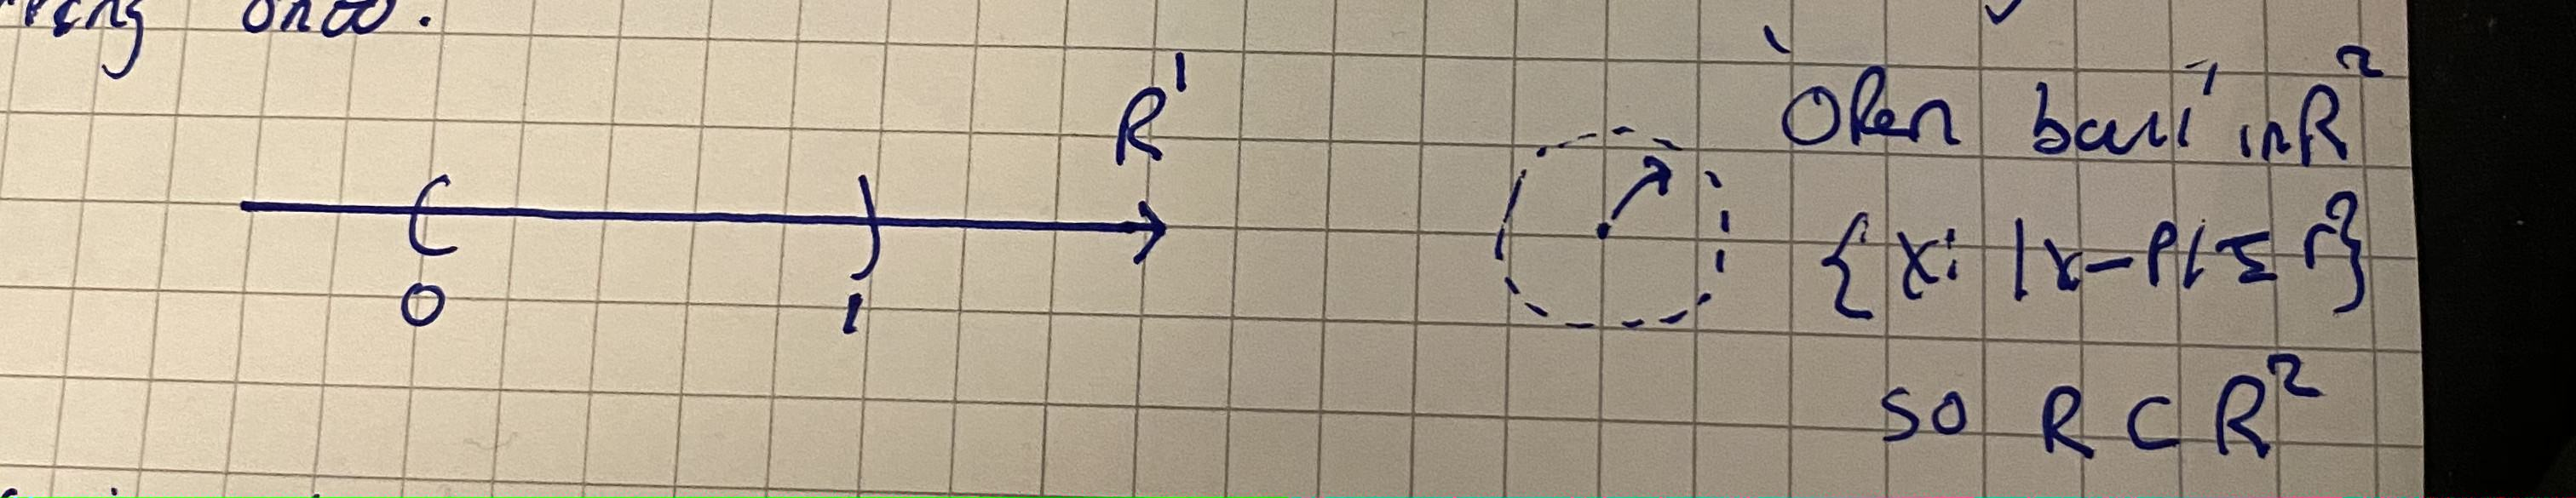
\includegraphics[width=8cm]{fig1.jpg}
  \centering
 \end{figure}
 \\
 \\
 The closed interval $I=[0,1]$ is clearly a manifold as it is homeomorphic to the extended real number line and is a subset of $\mathbb{R}^n$  with 
 $$ O_i: u_i \rightarrow \phi_i (U_i) \subset \mathbb{H}^1 $$
 The boundary points 0 and 1 are homeomorphic to $\mathbb{H}^1$ as there exists a bijection between them. 
 \item  $S^1=\defset{(\cos \varphi,\sin\varphi)}{\varphi\in \R}\subset \mathbb{R}^2$
 $$ M = S^1 \times I = S^1 \times [0,1] $$
Due to $S^1$ being a manifold and I being a manifold with a boundary, every point $(a,b) \in S^1 \times I$ will have an open set which is the product $p \times q$, which are subsets of $S^1$ and I, s.t $p \subseteq S^1, q \subseteq I$ and are open such that $a \in p, b \in q$. If we pick $p$ and $q$ where $p$ is homeomorphic to $\mathbb{R}^2$ and $q$ is homeomorphic to $\mathbb{H}^1$ then we can produce the mappings 
$$ f: p \rightarrow \mathbb{R}^2$$
$$ g: q \rightarrow \mathbb{H}^1$$
Which are both homomorphisms with a product mapping 
$$ F: p \times q \rightarrow \mathbb{H}^2$$ 
So $M$ is a manifold with a boundary. \\
Assuming continuity, M is homeomorphic to the tube or cylinder in $\mathbb{R}^3$ which would be given by the quotient space of $[0,1] \times [0,1]$, the unit square. This is because M could be mapped onto and one-to-one with the finite cylinder. 
\\
$S^1$ has dimension 1 and $[0,1]$ has dimension 1 so M must have dimension 2 as it is the product manifold. 
 \item Compute the manifold boundary $\partial M$. 
 Is it compact and/or connected?
 \\
 $S^1$ is a manifold without a boundary and I is a manifold with a boundary $\partial I$. So, M, has a boundary 
 $$ \partial M = \partial I \times \mathbb{R}^1 $$
 Which would be 0 dimensional (?). \\
 The topological space is connected as $S^1$ is connected and I is connected. The connectedness of I following from the fact that it is a subset of Real Numbers. The connectedness of $S^1$ is trivial but take the map 
 $$ f: [0,2 \pi] \rightarrow \mathbb{R}^2 $$
 So we have 
 $$ f(\theta) = (cos(\theta), sin(\theta)) $$
 Which is a continuous map. The interval $[0, 2\pi] $ is connected as it is a subset of $\mathbb{R}^n$ and the image of $f$ is $S^1$ which must be connected. 
 \\
 Also, $S^1$ cannot be written as $X_1 \cup X_2$ where $X_1$ and $X_2$ are open, empty disjoint sets and neither can $I = [0,1]$, reaffirming the previous statement. 
 \\
 $S^1$ is compacted as it is a closed and bounded subspace of $\mathbb{R}^2$. $I=[0,1]$ is compact as it is finitely coverable by an open cover, therefore $M=S^1 \times I$ is compact and connected.  
\end{alplist}


\end{document}

